\chapter{\label{ch:1-intro}Introduction} 

%\minitoc

\section{Overview}
...

% 1
\section{The adaptive immune system}
Humans are exposed to millions of potential pathogens every day and therefore require defences to be able to protect themselves against infection.
These defences can be innate or adaptive.
An example of an innate defence is the skin acting as a physical barrier between the outside world and the body.
Another example of an innate defence is non-specific engulfing (phagocytosis) of foreign pathogens by macrophages (a type of white blood cell).
Innate responses are relied upon as the first line of defence, however sometimes a more sophisticated, specialised response is required- called the adaptive immune response. (REF-mol biology of the cell).

Adaptive immune responses are specific to the pathogen that induced the response and are dependent on B cells and T cells, two major classes of lymphocytes (a class of white blood cell).
Two classes of adaptive immune responses exist: antibody responses, co-ordinated by B cells, and cell mediated immune responses, co-ordinated by T cells.
T-cell-mediated immune responses recognise foreign antigens (antibody generators;
substances capable of eliciting an immune response by stimulating B or T cell activation) on the surface of cells and can either kill the pathogen-infected cells or stimulate B cells or phagocytes to help eliminate the pathogen.
In antibody responses, B cells and plasma cells secrete antibodies, also known as immunoglobulins.
Immunoglobulins are large Y-shaped proteins, which recognise and bind to the specific foreign antigen on the pathogen which stimulated their production.
Binding of immunoglobulins to antigens renders the virus or microbial toxin inactive as it blocks their ability to bind to host cells.
Additionally, antibody binding makes it easier for phagocytic cells to ingest the pathogen.
%%%%%%


%2
\subsection{Plasma cells}
%3
\subsubsection{Plasma cell development}
Stem cells are precursor cells which can give rise to at least one type of differentiated (mature) cell, with the capability of indefinite self-renewal.
Hematopoietic stem cells (HSC) are stem cells that give rise to all the cells of the hematopoietic system.
Two predominant cell populations are produced by HSCs: the common myeloid progenitor (CMP) and the common lymphocyte progenitor (CLP).
CMP differentiation produces erythrocytes (red blood cells), mast cells, monocytes, macrophages, neutrophils, eosinophils, basophils and myeloid dendritic cells.
CLP differentiation results in B cells, T cells, natural killer (NK) cells and lymphoid dendritic cells.

%% Immune cell figure
\begin{figure}
\centering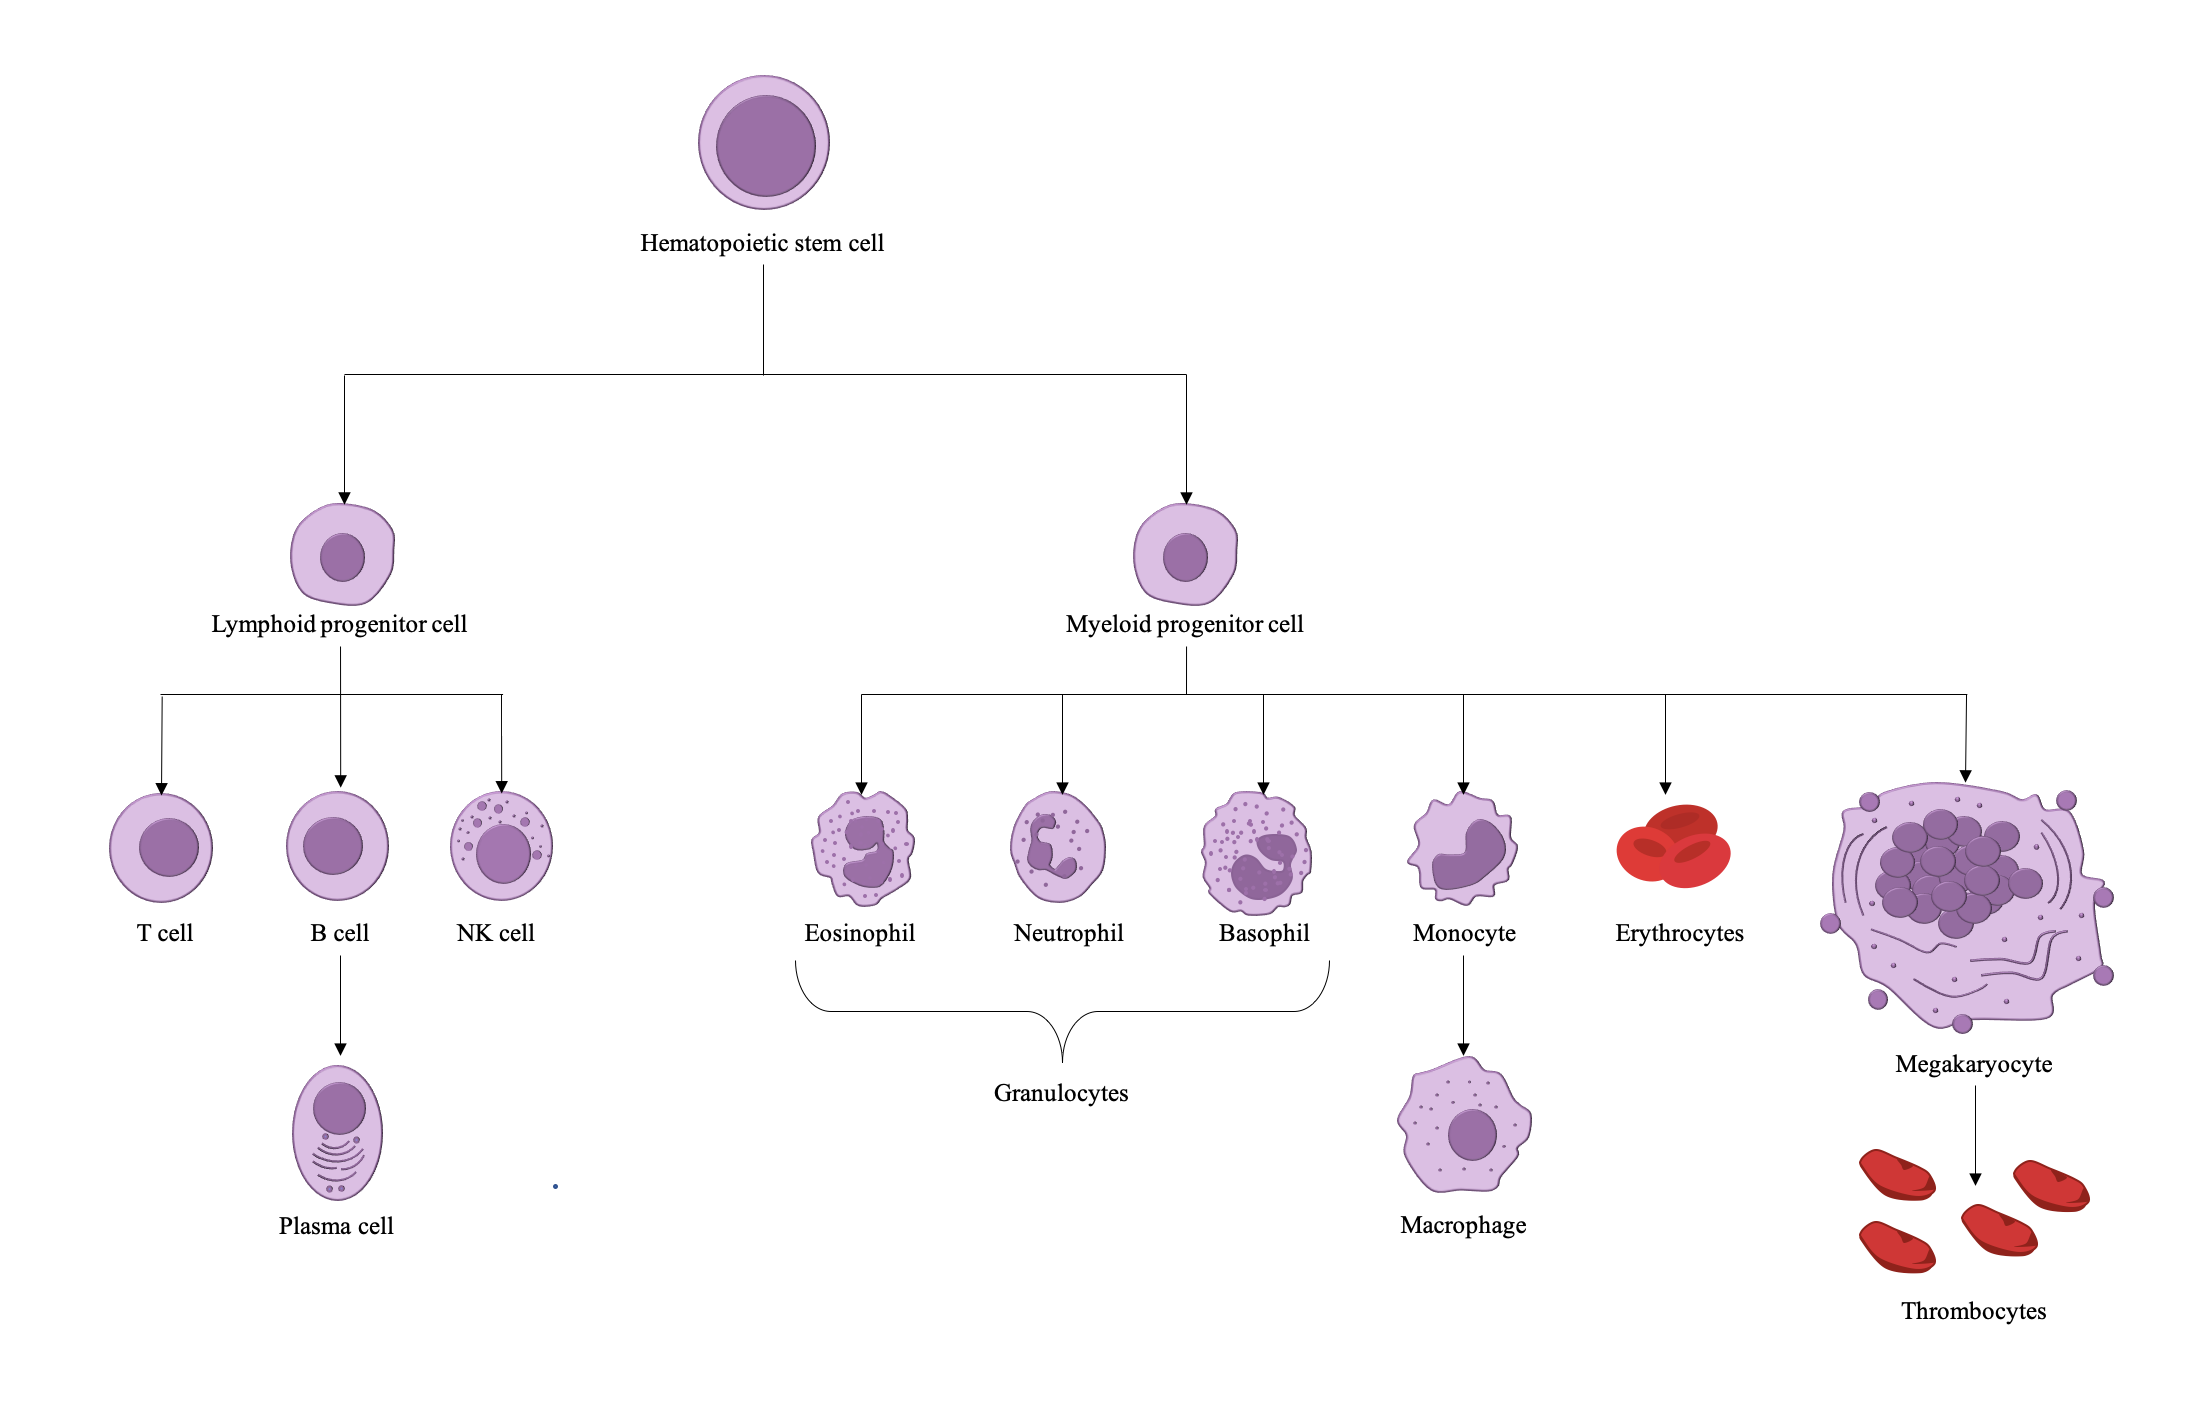
\includegraphics[width=0.7\textwidth]{figures/Introduction/immune_cells.png}
\caption[Hematopoietic system cell differentiation]{Hematopoietic stem cell (HSC) cell differentiation. HSCs divide into myeloid or lymphoid progenitor cells. Dendritic cells and a number of precursor states have been ommitted. }
\label{fig:HSC_differentiation}\end{figure}
%%

Most B cells die in the bone marrow soon after developing, however some will develop in the bone marrow, where initial stages of maturation occur and then migrate to secondary lymphoid organs, such as the spleen.
Within secondary lymphoid organs, numerous critical decisions on B cell fate are made, involving complex transcriptional networks, cell interactions, gene rearrangements, and mutations\cite{roth2014tracking, jourdan2011characterization}.
Upon antigenic-stimulation, naive B cells differentiate into memory B cells or plasma cells.
Terminally differentiated plasma cells are the final effectors of the B cell lineage, each dedicated to secreting large amounts of a single type of antibody.
Plasma cells have an extensive rough endoplasmic reticulum (ER), and have numerous genes involved in immunoglobulin secretion upregulated, including \textit{XBP-1} and \textit{CHOP}\cite{shapiro2004plasma}, to enable the production of copious amounts of antibody.
Plasma cells appear to consist of two distinct categories: short-lived plasma cells, which have life-spans of several months and are located in extrafollicular locales such as in medullary chords of lymph nodes or the red pulp of the spleen, and long-lived plasma cells, which have life-spans of decades and are mainly found in the bone marrow\cite{bortnick2013and, andraud2012living}.



%1
\section{Multiple myeloma}\label{sec:MM}
%2
\subsection{Multiple myeloma cells}
Multiple myeloma is a malignancy of terminally differentiated plasma cells.
It is characterised by aberrant proliferation of clonal, long-lived plasma cells in the bone marrow\cite{anderson2011pathogenesis}.
The large accumulation of MM cells in the bone marrow, crowd out healthy cells.
Under normal conditions, plasma cells produce antibodies that fight infection as part of the adaptive immune system.
However malignant plasma cells (MM cells) produce large amounts of abnormal antibodies that are unable to fight infection, coined `paraproteins' or `M proteins' (Figure \ref{fig:m_spike}).

%% M spike
\begin{figure}
\centering
\includegraphics[width=\textwidth]{figures/Introduction/M_spike.pdf}
\caption[M spike diagram]{Diagram of serum protein electrophoresis (SPEP) for a normal individual and for a multiple myeloma (MM) patient.
Based on their electrical charge, SPEP separates all the proteins in the blood.
A large peak is recorded for albumin (the most abundant protein in the blood), followed by lower levels of the other proteins, grouped into areas labelled $\alpha1$ and $\alpha2$, then a $\beta$ region, and then a $\gamma$ region, which represents where antibodies lie on the graph.
The large quantities of a single type of antibody (M protein) produced by MM cells cause a distinct `M spike' in the antibody protein region of the graph ($\gamma$ region).}
\label{fig:m_spike}
\end{figure}
%%

%2
\subsection{Epidemiology}
Multiple myeloma accounts for 1-2\% of all cancers and has the second highest incidence of hematological malignancies, after non-Hodgkin's lymphoma\cite{international2003criteria}.
MM is rare in individuals under the age of 40, with the average age at time of diagnosis centering around 70\cite{tsang2019multiple, palumbo2011multiple}.
MM is more prevalent in males than females and is around twice as common in black populations than in Caucasian or Asian populations\cite{nhsmyeloma}.
The average incidence rate is approximately 1-6 cases per 100,000 individuals\cite{tsang2019multiple, palumbo2011multiple, teras20162016}, with the highest age-standardised incidence rates in the regions of Australasia, North America, and Western Europe\cite{cowan2018global}.
Five-year survival rate of MM patients is approximately 49\%, whilst approximately a third of MM patients survive ten years or greater\cite{cancerresearchuk, siegel2016cancer}.
%While there have been many successful medicines developed for myeloma, they all suffer from the development of drug resistance.

%2
\subsection{Presentation}
%3
\subsubsection{Precursor states}
All cases of MM are preceded by asymptomatic precursor states, monoclonal gammopathy of unknown significance (MGUS) and smoldering multiple myeloma (SMM).
However, only some patients with SMM or MGUS progress to active MM.

MGUS is a pre-malignant condition where patients have the presence of monoclonal immunoglobulins in their blood or urine, $<$10\% clonal plasma cells in their bone marrow, but lack any myeloma-related end-organ damage\cite{van2018mgus}.
Patients with SMM have between 10 and 60\% clonal plasma cells in their bone marrow, serum monoclonal immunoglobulin of $\ge$3 g/dL, and like MGUS, have no signs of end-organ damage\cite{rajkumar2015smoldering}.
Progression risk of MGUS into symptomatic MM is about 1\% per year, whilst progression risk of SMM to MM is higher, at around 10\% per year for the first 5 years, after which it decreases\cite{korde2011monoclonal, kyle2007clinical}.
%

%3
\subsubsection{Active MM}
There are multiple classifications of active MM.
The International Myeloma Working Group's definition\cite{rajkumar2014international} is as follows:
Greater than 10\% clonal plasma cells located in the bone marrow and one or more myeloma-defining event or biomarker of malignancy.
Myeloma defining events consist of evidence of end-organ damage that can be attributed to the surplus of M protein and clonal plasma cells, namely the CRAB features:
%
% List of myeloma events (CRAB)
\begin{itemize}
  \item Hypercalcemia
    \begin{itemize}
        \item Serum calcium $>$ 1 mg/dL higher than the upper limit of normal, or
        \item Serum calcium $>$ 11 mg/dL
    \end{itemize}
  \item Renal insufficiency
    \begin{itemize}
        \item Creatinine clearance $<$ 40 mL per min, or
        \item Serum creatine $>$ 2 mg/dL
  \end{itemize}
  \item Anemia
    \begin{itemize}
        \item Hemoglobin value of $>$  20 g/L below the lower limit of normal, or
        \item Hemoglobin value $<$ 100 g/L
    \end{itemize}
    \item Bone lesions
      \begin{itemize}
        \item One or more osteolytic lesions on skeletal radiography, CT or PET-CT
        \end{itemize}
\end{itemize}
% End of list
%

Biomarkers of malignancy include greater than or equal to 60\% clonal plasma cells in the bone marrow, an involved:uninvolved serum free light chain ratio greater than or equal to 100, and more than one focal lesion on an MRI study\cite{rajkumar2014international}.

%
It is currently unclear what causes the malignant transformation between precursor states and active MM\@.
However certain factors have been identified as risk factors, including point mutations, a large array of up-regulated transcription factors, and numerous immune events.

\subsection{Treatment of multiple myeloma}\label{subsec:mm_treatment}
Multiple myeloma may be an incurable disease, however it is treatable.
In fact, in the last decade median survival time for newly diagnosed MM patients has almost doubled\cite{kazandjian2016look}.
Novel therapeutic advances have contributed to this improvement (Table \ref{tab:treatment_history}).
Myeloma is usually treated with a combination of drugs, often comprising a corticosteriod, a proteasome inhibitor, and an immunomodulatory drug (IMiD).
A common regimen, approved in the USA, European Union and UK for untreated myeloma is the triplet VRd regimen.
This consists of the proteasome inhibitor bortezomib (brand name Velcade), the IMiD lenalidomide (brand name Revlimid), and the corticosteroid dexamethasone.

% Timeline of treatment options
%% Table for treatment timeline


\begin{table}[h]
\centering
\begin{tabular}{|p{1cm}|p{3cm}|p{8cm}|p{1.3cm}|}
\hline
\textbf{Year} & \textbf{Treatment} & \textbf{Usage} & \textbf{Ref} \\ \hline
1958 & Melphalan & The alkylating agent melphalan was first used in plasma cell myeloma in 1958. & \cite{blokhin1958clinical} \\ \hline
1960s & Corticosteroids & Placebo-controlled double-blind trial of prednisone in multiple myeloma. Combinations of prednisone and melphalan showed an increased survival over melphalan alone. Dexamethasone and prednisone have become a cornerstone in the treatment of multiple myeloma. & \cite{mass1962comparison, alexanian1969treatment} \\ \hline
1980s & Stem-cell transplantations & Numerous successful allogenic and autologous bone marrow transplantations in patients with multiple myeloma &  \cite{mcelwain1983high, osserman1982identical, fefer1986identical, gahrton1987bone}  \\ \hline
2003 & Proteasome inhibitors & Bortezomib, a first-in-class proteasome inhibitor, was first approved by the FDA for use in relapsed and refractory multiple myeloma. In 2008 it was approved for patients with no prior treatment. Carfilzomib was approved in 2012 for advanced MM and later in 2015 for treatment of relapsed MM. The oral proteasome inhibitor, ixazomib, was approved as a combination treatment with lenalidomide and dexamethasone in 2016 for people who have received at least one previous treatment. & \cite{kane2003velcade,richardson2003phase,katsnelson2012next} \\ \hline
2006 & IMiDs & The antitumour activity of thalidomide was demonstrated in 1999, this led to the development of lenalidomide, the first approved immunomodulatory imide drug (IMiD) for use in multiple myeloma. Currently, thalidomide, lenalidomide and pomalidomide are approved for use in multiple myeloma & \cite{singhal1999antitumor,label47revlimid,san2013pomalidomide} \\ \hline
2015 & Monoclonal antibodies & In 2015, daratumumab, an anti-CD38 monoclonal antibody and elotuzumab, an anti-SLAMF7 monoclonal antibody, were approved for MM treatment. & \cite{lokhorst2015targeting,lonial2015elotuzumab} \\ \hline
\end{tabular}
\caption[Timeline of treatment options for multiple myeloma]{Timeline of treatment options for multiple myeloma. Listed by first usage or FDA approval for MM.}
\label{tab:treatment_history}
\end{table}

% https://www.ncbi.nlm.nih.gov/pmc/articles/PMC5282737/
% https://www.ncbi.nlm.nih.gov/pmc/articles/PMC2265446/
% Panobinostat	HDACi
% Liposomal doxorubicin	DNA inter-calator



\subsection{Proteasome inhibitors}
Proteasome inhibitors have contributed greatly to the improved prognosis of MM since their introduction into treatment regimes.
The first-in-class proteasome inhibitor bortezomib (Velcade\textsuperscript{\textregistered}) was approved by the FDA in 2003 as a single-agent for injection of relapsed MM\cite{kane2003velcade}.
Since then it has been approved for use in combination therapies.
Bortezomib in combination with melphalan-prednisone proved to be superior to the previous standard of care for patients ineligible for HDT-ASCT of melphalan-prednisone alone, increasing time until tumour progression\cite{san2008bortezomib}.
The combination of bortezomib, dexamethasone and thalidomide  was also shown to be superior to previous standard of care for patients prior to ASCT\cite{moreau2012proteasome}.
In 2010, bortezomib was approved as a frontline therapy for treatment-naive MM patients.
Since then, two more proteasome inhibitors have been approved, carfilzomib and ixazomib.
Carfilzomib is structurally and mechanistically different to bortezomib and shows activity on bortezomib resistant primary MM cells\cite{moreau2012proteasome}; it is approved for relapsed or refractory MM\@.

\subsubsection{The ubiquitin-proteasome system}
Proteasome inhibitors work by blocking the action of the proteasome in the cell.
Misfolded proteins can be harmful to a cell, so the combined activity of molecular chaperones, which aid in protein folding, and the ubiquitin-proteasome system (UPS), which acts to digest misfolded proteins, is needed to prevent massive protein aggregation.
Unneeded, misfolded or damaged proteins are tagged with lysine-48-linked poly-ubiquitin chains, marking them for degradation by the proteasome (Figure \ref{fig:26s_proteasome_structure}).
The proteasome is sometimes described as a complex `protein destruction machine'.
The proteasome consists of the 20S core particle, a central hollow cylinder, and the 19S regulatory caps associated with each end of the cylinder.
The 19S regulatory caps perform substrate recognition, deubiquitination, unfolding and threading of the protein substrate into the 20S core.
The core is made up of four stacked heptameric ring structures.
The outer rings are responsible for docking to the 19S cap and for acting as a gate to the inner rings. The inner rings consist of seven $\beta$ subunits, containing inward-facing protease active sites for degrading proteins\cite{kleiger2014perilous, alberts2007molecular} (Figures \ref{fig:26s_proteasome_structure} and  \ref{fig:proteasome_beta_subunits}).

 % Proteasome structure diagram
\begin{figure}[ht]
%1
\begin{subfigure}[t]{0.5\textwidth}
    \includegraphics[width=\textwidth]{figures/Introduction/26s_proteasome_serif.jpg}
    \caption{26S proteasome}
    \label{fig:26s_proteasome_structure}
\end{subfigure}
%\medskip
\begin{subfigure}[t]{0.5\textwidth}
    \includegraphics[width=\textwidth]{figures/Introduction/20s_core_beta_subunits_serif.jpg}
    \caption{$\beta$-subunits of an inner ring of the 20S core particle }
    \label{fig:proteasome_beta_subunits}
\end{subfigure}
    \caption[Structure of the proteasome]{Structure of the proteasome. \ref{fig:26s_proteasome_structure} shows the structure of the 26S proteasome, comprised of the 19S regulatory caps and 20S core particle.
    A misfolded protein tagged with a poly-ubiquitin chain is recognised by the 19s regulatory cap, which cleaves the ubiquitins from the protein and threads the protein through to the core, where it is degraded into small peptides.
    The 20S core particle is made up of two outer rings of $\alpha$-subunits and two inner rings of $\beta$-subunits.
    \ref{fig:proteasome_beta_subunits} shows the $\beta$-subunit arrangement in one of the inner rings of the 20s particle.
    $\beta1$ (caspase-like), $\beta2$ (trypsin-like) and $\beta5$ (chymotrypsin-like) are the proteolytically active subunits.
    Proteasome inhibitors are designed to primarily inhibit $\beta5$.}
\label{fig:proteasome_and_beta}
\end{figure}

\subsubsection{Mechanism of action}
Of the seven proteasome $\beta$ subunits, only $\beta1$, $\beta3$ and $\beta5$ are proteolytically active (Figure \ref{fig:proteasome_beta_subunits}). Proteasome inhibitors are designed to target $\beta5$ as it has been shown as the rate limiting protease for proteasomal protein turnover \cite{besse2019proteasome}. Bortezomib reversibly co-inhibits $\beta5$ and $\beta1$ subunits, whilst carfilzomib irreversibly binds to $\beta5$, with greater selectivity than bortezomib, and at higher doses binds to $\beta2$ as well \cite{besse2019proteasome}.


The precise downstream effects of $\beta$ subunit proteasome inhibition are not fully understood, however the unfolded protein response (UPR), NF-$\kappa$B signalling, JNK signalling, apoptotic factors and p53 are thought to be involved in the anti-MM effects \cite{kubiczkova2014proteasome}.
Specifically, the action of the UPR has been demonstrated as an important mechanism in the anti-MM effect of PIs.
MM cells secrete large amounts of monoclonal protein, leading to the rapid accumulation of  misfolded proteins within the endoplasmic-reticulum (ER) lumen.
This results in heightened ER stress, which is compensated by the UPR by reducing global protein translation and up-regulating UPS machinery \cite{wallington2018resistance}.
Therefore, by inhibiting the proteasome, fewer ubiquitin tagged proteins are degraded and more misfolded proteins accumulate in the ER lumen.
ER stress is then further increased, causing the UPR to switch from a homeostatic, pro-survival system to a pro-apoptotic pathway \cite{kubiczkova2014proteasome, wallington2018resistance}.

Another important mechanism for PI is the attenuation of NF-$\kappa$B signalling. I$\kappa$B$\alpha$, a specific endogenous inhibitor of the transcription factor NF$\kappa$B, is a protein degraded by the proteasome.
Inhibition of the proteasome increases levels of I$\kappa$B$\alpha$, thereby abolishing NF$\kappa$B signalling.
NF$\kappa$B is a key transcription factor in many cancers, contributing to overall tumour growth and chemoresistance.
NF$\kappa$B has been shown to promote tumour cell proliferation, anti-apoptotic and angiogenic factors \cite{kale2012molecular}.

\section{Drug resistance in multiple myeloma}
Although PIs are extremely effective at killing MM cells initially, long-term treatment inevitably results in a drug-resistant relapse.
Drug resistance is one of the biggest barriers in the treatment of MM.
Patients follow a pattern of peaks and troughs of treatment cycles, remission and relapse, until all therapies have little effect (Figure \ref{fig:treatment_cycles}).
%% Treatment cycles
\begin{figure}[htb]
\centering
\includegraphics[width=\textwidth]{figures/Introduction/treatment_cycles.pdf}
\caption[MM treatment cycles]{MM treatment cycles and disease progression over time.
All MM patients begin with precursor states Monoclonal Gammopathy of Unknown Significance (MGUS) and/or smoldering multiple myeloma (SMM) prior to a malignant transformation to symptomatic/active MM.
Patients undergo cycles of treatment, remission and relapse until eventually becoming relapsed and refractory (RRMM) and no longer respond to treatment.
}
\label{fig:treatment_cycles}
\end{figure}
%%
In order to overcome resistance and increase overall survival of MM patients, the molecular mechanisms of resistance to proteasome inhibitors needs to be understood.
This  will aid in the design of novel therapies and inform better use of existing therapies.
Previous studies on proteasome drug resistance have been performed and certain mechanisms and genes have been identified.
For example, point mutations have been noted in the \textit{PSMB5} gene (coding for the $\beta5$ subunit of the proteasome), as well as and over-expression of the $\beta5$ subunit \cite{robak2018drug}.
Other upregulated genes have been identified, for example \textit{ABCB1}, coding for P-glycoprotein, responsible for pumping various substrates out of the cell, also referred to as multidrug resistant protein 1.
\textit{XBP1}, involved in the UPR, has been seen to be downregulated in PI resistance \cite{robak2018drug}.
Although many genes have been identified to be differentially expressed in drug resistant MM, the mechanism is not fully elucidated and further research is imperative in the progression of treatment for multiple myeloma.

Another avenue to increase MM survival, would be to identify novel therapeutics effective against MM, which are capable of overcoming acquired anti-cancer drug resistance.
By increasing the arsenal of drugs available to treat MM, the time until patients become refractory and no longer respond to treatment could be prolonged.
Therapeutics with a novel mechanism of action are likely to be more effective for MM patients who have undergone several treatment cycles than drugs belonging to the same class as drugs they have previously been treated with.
Novel therapeutics would have less overlap of mechanism of action with existing drugs, therefore there would be less cross-resistance.

%
\afterpage{\clearpage} % flush out floats before this. Very different section
%
\section{Transcriptomics, proteomics and epigenomics}
It has been shown that changes in the genome, transcriptome, epigenome and proteome all contribute to disease progression and drug resistance in MM.
Therefore, to sufficiently investigate the multiple layers driving MM and to assess the effectiveness of new therapeutics, a multi-omics approach must be employed.

\subsection{DNA and the genome}\label{subsec:dna}
The genome is the genetic material of an organism, it consists of deoxyribonucleic acid (DNA).
DNA consists of two polynucleotide chains (or strands), running anti-parallel to each other, held together in a double helix structure by hydrogen bonds.
Nucleotides are composed of a five-carbon sugar (deoxyribose for DNA), attached to one or more phosphate group (a single phosphate group in the case of DNA) and a nitrogenous base.
Nucleotides are covalently linked to form an alternating sugar-phosphate backbone, with bases extending from each sugar towards the inside of the double helix.
Nucleotides contain four different types of bases: adenine (A), cytosine (C), guanine (G) and thymine (T).
The two DNA chains are held together by hydrogen bonds via complementary base pairing between the bases of the strands, A pairing with T and G pairing with C\@.
Often sections of DNA are denoted as their sequence of A, C, T and Gs (in order reading from the 5' to 3' direction).

Every individual has approximately 6 billion base pairs of DNA per cell, which would amount to about 2 metres of DNA if laid end-to-end.
The nucleus of a human cell is approximately 6\si{\micro\meter} in diameter, therefore chromosomal DNA must be folded tightly to fit.
DNA packaging is a complex task involving numerous speciliased proteins.
Negatively charged DNA is complexed with an octomer of positively charged proteins called histones to form nucleosomes.
The histone core is made up of eight subunits, two copies of H2A, H2B, H3 and H4 subunits.
DNA wraps tightly around the histone core 1.65 times.
Linker DNA connects adjacent nucleosomes, to resemble `beads on a string'.
Nucleosomes fold tightly to form 30\si{\nm} chromatin fibre, which in turns forms loops averaging 300\si{\nm} in length.
This fibre is folded and compressed again to form fiber 250\si{\nm} in width with loops of 700\si{\nm} in length.
Tight coiling of this fiber forms the single chromatids of chromosomes \cite{annunziato2008dna, alberts2002chromosomal}.
Human cells contain 23 pairs of chromosomes.

% DNA structure and packaging
\begin{figure}[htb]
%1
\begin{subfigure}[t]{0.5\textwidth}
    \includegraphics[width=\textwidth]{figures/Introduction/nucleotides_dna_helix.png}
    \caption{Nucleotide and DNA double helix structure}
    \label{fig:base_pairs}
\end{subfigure}
%\medskip
\begin{subfigure}[t]{0.5\textwidth}
    \includegraphics[width=\textwidth]{figures/Introduction/dna_packaging.png}
    \caption{DNA packaging}
    \label{fig:DNA_packaging}
\end{subfigure}
    \caption[DNA stucture and packaging.]{\ref{fig:base_pairs} shows the DNA nucleotides and the DNA double helix structure.
    DNA consists of two polynucleotide chains.
    Nucleotides are covalently linked to one another, forming a sugar-phosphate backbone.
    They contain one of four bases adenine (A), cytosine (C), guanine (G) and thymine (T).
    DNA strands are held together by hydrogen bonds between complementary base pairs, A pairing with T and G pairing with C\@.
    Sections of DNA are are often read by their sequence of bases from the 5' direction to the 3' direction.
    \ref{fig:DNA_packaging} shows how chromosomal DNA is packaged in the cell.
    DNA wraps 1.65 times around an octomer of histone proteins, to form a stucture called a nucleosome.
    Nucleosomes are linked by linker DNA to form a structure that resembles `beads on a string'.
    Nucleosomes fold to create chromatin fiber.
    This is turn forms loops and coils tighter and tighter until it makes up the single chromatids of chromosomes.
    \\\hspace{\textwidth}Created with BioRender.com.
    }
\label{fig:DNA_structure_packaging}
\end{figure}

The complete genome is made up of coding DNA (genes), non-coding DNA, as well as mitochondrial DNA and ribosomal DNA\@.
An alteration in the nucleotide sequence of the genome is called a mutation.
There are a number of types of mutations, including insertions, deletions, inversions, substitutions and duplications.
A technique called whole genome sequencing (WGS) can be used to determine the sequence of nucleotides in an individual's DNA and therefore it can be used to determine any variations in the genome.
% However the technique is expensive and many experiments are interested in coding DNA only, so perform RNA-seq to look at the transcriptome instead.

% Diagram double helix with bases in the middle. Then one of sequence of ACTG etc.
% Diagram of DNA genes transcribed to RNA then translated to proteins (pg 301 of textbook is good example)

\subsection{The epigenome}
Epigenetics is the study of any heritable phenotypic changes that do not involve alterations of the DNA sequence itself.
These changes occur at the chromatin level.
Epigenetic changes include histone modifications, DNA methylation and chromatin remodelling.
%These epigenetic changes are described in more detail below.

DNA methylation is the addition of methyl groups to the C5 position of cytosines in DNA.
This happens extensively at CpG sites (cytosine followed by a guanine).
Stretches of DNA with a high CpG ratio (CpG islands) are often found in the promoter region of genes.
Increased DNA methylation at CpG islands results in transcriptional silencing of those genes.
Genome wide DNA methylation is often examined using DNA-methylation-seq or DNA methylation microarrays.

DNA wraps tightly around histones (section \ref{subsec:dna}), they contribute to the tight packaging of DNA.
Histone modifications are post-translational modifications.
They include methylation, acetylation, phosphorylation, ubiquitination and sumoylation.
Histone modifications affect transcriptional activity either by directly influencing the structure of chromatin and DNA accessibility or by regulating binding of effector molecules to `read' histone marks to mediate downstream biological effects.
Histone modifications also regulate DNA processes, such as repair, replication and recombination \cite{ bannister2011regulation}.
Chip-seq can be used to investigate and measure various post-translational histone modifications.

Chromatin remodelling is the process of modifying chromatin architecture to regulate the accessibility of DNA.
Gene expression is regulated by allowing certain gene regions better access to transcription machinery.
This is achieved by ATP-dependent chromatin-remodelling complexes moving, ejecting or restructuring nucleosomes.
ATAC-seq can be used to identify accessible DNA regions.


\subsection{The transcriptome}
Transcription is the first of many steps in gene expression.
During transcription, the enzyme RNA polymerase reads a DNA sequence and produces an anti-parallel, complementary ribonucleic acid (RNA) strand.
The transcriptome is the set of all RNA transcripts of an individual.
RNA is a nucleic acid similar to DNA. Like DNA it has a sugar-phosphate backbone and 4 different types of bases attached to each sugar.
However, unlike DNA, RNA is single-stranded, it contains the sugar ribose in place of deoxyribose, and the nucleotide uracil (U) inplace of thymine (T).

Despite the chemical differences between DNA and RNA, they are essentially written in the `same language' and one-to-one mapping of nucleotides can be performed.
Transcription begins with the unwinding and opening of a small part of the DNA double helix, so bases are exposed.
One strand of DNA acts as a template and the RNA chain is formed by complementary base pairing with the template.
RNA polymerases catalyse the reaction of forming phosphodiester bonds between nucleotides, forming the RNA chain.
The RNA polymerase moves stepwise along the DNA chain, unwinding the chain just ahead exposing a new region of the template strand.
Just behind the region where ribonucleotides are being added, the DNA helix reforms.

The genes in a cell's DNA that specify the amino acid sequence and result in protein synthesis are called messenger RNA (mRNA) molecules.
Genes that produce the RNA molecule itself are called non-coding RNAs, because they do not code for proteins.
There are many other types of RNA, such as transfer RNA (tRNA), ribosomal RNA (rRNA) and micro RNA (miRNA).

Traditionally microarrays were used to measure gene expression.
Now RNA-seq (outlined in section  \ref{subsec:rna-seq-intro}) is more commonly used study to gene expression and the transcriptome.
Depending on the library preparation, different types of RNAs can be selected for or excluded, to study different RNA molecules.

\subsection{The proteome}\label{subsec:translation}
The proteome is the entire set of proteins that is or can be expressed by an organism.
mRNAs are translated into protein molecules.
mRNA is made up of only four different nucleotides, but proteins are made up of 20 amino acids, therefore a direct one-to-one function matching nucleotides to amino acids is impossible.
Instead, the sequence of mRNA is read in groups of three consecutive nucleotides, called a codon.
The three positions of a codon, and each position with four possible base options (A, C, U and G), gives a total of 64 different permutations (i.e. 4\textsuperscript{3}).
Therefore, some combinations map to the same amino acid (many-to-one function), or signal to terminate translation of the current protein, named a stop codon.
This genetic code directs the translation from mRNA to protein.
Translation takes place in the ribosome.

Codons on mRNA do not directly recognize their given amino acid, they require tRNA molecules that bind to both the codon on mRNA and the correct amino acid.
tRNAs possess an anticodon, a set of three nucleotides complementary to a given codon.
Firstly, tRNAs are coupled to their cognate amino acid.
This reaction is catalysed by aminoacyl-tRNA synthetase (aaRS) enzymes.
aaRSs attach amino acids to the 3' end of tRNA.
Most cells have a specific aaRS for each amino acid.
Once the tRNA is charged with the correct amino acid, the tRNA molecule binds to its complementary codon on mRNA.
Subsequent aminoacylated tRNA molecules bind to mRNA codons.
A polypeptide chain grows by stepwise addition of amino acid to the C-terminal end.
The formation of the new peptide bond between amino acids releases the tRNA molecule.
The peptide chain grows until a stop codon is reached and synthesis of the current protein is complete.

Protein translation is partly regulated by availability of mRNAs, but it also depends on other factors such as RNA silencing and post-transcriptional modifications.
Proteins have a large array of functions, such as transporting small molecules, catalysing reactions, cell-cell signalling and providing structural support.

Proteomics is the study of the proteome.
CyTOF and LC-MS/MS are techniques often employed to examine the proteome. %(section \ref{subsec:cytof-intro} and section \ref{subsec:lcmsms-intro}).

\subsection{Sequencing}
DNA is often referred to as the `genetic master code', therefore the ability to decode the order of nucelic acids has been seen as a highly desirable feat since its discovery.
Sequencing is the process of determining the sequence of nucleotides of nucleic acid residues.
Over the last half-century, large numbers of researchers and vast sums of money have been applied to facilitate the techniques and technologies to decode DNA and RNA molecules' nucleotide sequence \cite{heather2016sequence}.
Over this time, massive technological innovations have been developed.
The most commonly used `first-generation' DNA-sequencing technology, Sanger sequencing, was developed in 1977 \cite{sanger1977dna}.
In Sanger sequencing, or the `chain termination method', chain-termination PCR is performed with a mix of regular nucleotides (deoxynucleotide triphosphates; dNTPs) and fluorescently-labelled, chain-terminating dNTPs (dideoxynucleotide triphosphates; ddNTPs), using the DNA of interest as a template.
During the extension step of PCR, when DNA polymerase incorporates a ddNTP randomly, extension ceases.
This creates greater than a million copies of the DNA sequence of interest, all terminated at random lengths by the ddNTPs.
Capillary gel electrophoresis is then used to separate the extension products by size.
The gel is then read to determine the sequence.
By reading the gel bands from smallest to largest, the 5' to 3' sequence of the original DNA strand can be inferred.
Sanger sequencing was used by the Human Genome Project, an international research effort to determine the DNA sequence of the entire human genome \cite{pennisi2001human}.
The whole project took approximately 13 years to complete, and was reported to have cost \$3 billion.

Sanger sequencing dominated the sequencing world for over 30 years, until the advent of `Next-generation sequencing' (NGS; now being dubbed `second-generation sequencing', with the advent of newer technologies).
NGS differs from its predecessors in that it is highly scalable and massively parallel.
With NGS you can rapidly sequence the entire human genome in one day, for just under \$5000.
It is quicker and cheaper than traditional Sanger sequencing, and has progressed data output from the kilobase range up to potentially multiple terabases per run.
Today, the largest and most commonly used NGS sequencing technology platform is Illumina, who own around 80\% of the global sequencing market.
NGS can be used to study the transcriptome, using RNA-seq techniques (Section \ref{subsec:rna-seq-intro}); the epigenome, using techniques such as ChIP-seq or ATAC-seq; or the genome using techniques such as whole genome sequencing (WGS).

Recently, long-read technologies are becoming more prominent in the sequencing field.
Illumina short-read sequencing limits read length to between 50 and 300 base pairs (bp)\@.
This read length is too short to detect more than 70\% of human genome structural variation.
Moreover, some of the most mutation-prone regions of the genome are inaccessible due to repeating or GC-heavy content, limiting sequence coverage and leaving large regions of the genome critically understudied \cite{logsdon2020long}.
Long-read technologies are capable of generating continuous sequences ranging from 10 kilobases to several megabases, enabling the sequencing of full-length transcripts.
The two main emerging long-read technologies are PacBio single-molecule real-time (SMRT) sequencing\cite{wenger2019accurate} and Oxford Nanopore Technologies (ONT) sequencing\cite{ip2015minion, jain2016oxford}, together marking the birth of `third-generation sequencing' (TGS).
Both PacBio and ONT sequencing sequence single DNA molecules, rather than a pool of PCR-amplified fragments.
PacBio sequencing employs a sequencing-by-synthesis strategy (similar to Illumina sequencing), with circular DNA templates to improve accuracy.
ONT sequences a native linear single-stranded DNA molecule by measuring current changes as bases are threaded through a nanopore \cite{weirather2017comprehensive}.
Whilst TGS technologies have the advantage of longer read length, the methods are also plagued by higher base-calling error rates and lower throughput than NGS technologies \cite{weirather2017comprehensive, philpott2021nanopore}.
Therefore, this makes applying TGS to single-cell RNA-seq especially challenging.
Due to the lower through-put, fewer cells can be reported on at a comparable read-depth to NGS technologies;
and due to the high base-calling error rate, inaccurate cellular and molecular barcode assignment can complicate associating mRNA reads with their cell of origin.

\subsection{RNA-seq}\label{subsec:rna-seq-intro}
Most modern RNA sequencing (RNA-seq) implements NGS technology to analyse RNA across the transcriptome of a biological sample and allows for the quantification of gene expression.

\subsubsection{Bulk RNA-seq}
Bulk RNA-seq measures the average expression across a sample.
Creating a bulk RNA-seq library involves isolating RNA from a biological sample, filtering for a specific type of RNA (most commonly mRNA), fragmentation of RNA into fragments, reverse transcription of the fragments to generate a complementary DNA (cDNA) library, end repair and adaptor ligation of the cDNA library, followed by PCR amplification ready for sequencing.

%% Diagram of bulk RNA-seq
\begin{figure}[ht]
\centering
\includegraphics[width=0.8\textwidth]{figures/Introduction/bulk_rna_library_prep_diagram_alternate.png}
\caption[Bulk RNA-seq outline]{Outline of bulk RNA-sequencing library prep.
Cells are lysed and RNA is extracted.
The specific RNA of interest is selected and enriched, for example selecting for mRNA using polyA selection or ribo-depletion.
The mRNA is fragmented into smaller pieces of RNA.
First and second stranded cDNA are reverse transcribed from the RNA fragments using random primers.
The ends of the cDNA are repaired and dAMP (dA) tails are added to the 3' end of the DNA.
Adaptors are ligated to the 3' and 5' end of the cDNA.
These adaptors contain complementary sequences that allow the fragments to hybridize to the flow cell during sequencing.
Universal (P5/i5) and index (P7/i7) primers are added to the adaptor ligated DNA.
The libraries are then amplified using PCR and cleaned-up, ready for sequencing.
}
\label{fig:bulk_diagram}\end{figure}
%%

\subsubsection{Single-cell RNA-seq}
Single-cell RNA-seq (scRNA-seq) measures gene expression for each individual cell across a population of cells and therefore provides information on clonal diversity that may be lost when pooling cells into bulk samples.
Since its inception in 2009\cite{tang2009mrna}, there have been numerous scRNA-seq techniques developed, such as SMART-seq2\cite{picelli2013smart}, Drop-seq\cite{macosko2015highly}, STRT\cite{islam2011characterization}, scCOLOR-seq\cite{philpott2021nanopore} and inDrops\cite{klein2015droplet}.
scRNA-seq library preparation shares many steps with bulk RNA-seq workflow, however preliminary steps are required to isolate single cells and barcode reads that originated from the cell.
%% Diagram of drop-seq
\begin{figure}[hb]
\centering
\includegraphics[width=0.7\textwidth]{figures/Introduction/drop_seq.png}
\caption[Drop-seq schematic]{Outline of Drop-seq, a droplet-based scRNA-seq method.
A microfluidic device combines two aqueous flows, one containing cells and the other containing barcoded primer beads suspended in lysis buffer.
The two aqueous channels flow across an oil channel to form aqueous droplets surrounded by oil.
Relatively few droplets contain both a cell and a bead.
Following droplet formation, the cell is lysed and its mRNAs are released, which then hybridise to the primers on the bead surface.
A reagent is added to break up the droplets and the beads are collected and washed.
The mRNAs are reverse-transcribed into cDNAs, generating a set of ``STAMPS'' (single-cell transcriptomes attached to microparticles) and template switching is used to introduce a PCR handle.
The barcoded STAMPS can then be amplified using PCR.}
\label{fig:dropseq}\end{figure}
%%
For droplet-based scRNA-seq (dscRNA-seq) methods, single cells are isolated using microfluidic devices by individually encapsulating them in aqueous droplets contained in oil.
Below, a dscRNA-seq method, Drop-seq, is outlined (Figure \ref{fig:dropseq}).


% \subsection{ATAC-seq}

%\subsection{ChIP-Seq}
%Chromatin immunoprecipitation sequencing (ChIP-seq) is used to analyse protein interactions with DNA.
%At a base-pair resolution, it is used to map DNA-binding proteins and histone modifications.
%Therefore ChIP-seq is often used to determine the the mechanisms of gene regulation of transcription factors, and to study epigenetic mechanisms in detail.
%It utilises NGS to identify biding sites of DNA-associated proteins, therefore it is often used to determine the mechanisms of transcription factors or chromatin-associated proteins, influencing gene expression.


%\subsection{CyTOF}\label{subsec:cytof-intro}


%\subsection{Liquid chromatography with tandem mass spectrometry}\label{subsec:lcmsms-intro}
%Liquid chromatography with tandem mass spectrometry (LC-MS/MS) based proteomics is a popular analytical technique to measure the protein abundance of a sample.
%The general steps for LC-MS/MS-based proteomics include: cell lysis, protein extraction, protein digestion using an enzyme to cleave proteins into peptides, peptide purification, and analysis by mass spectrometry.
%The resultant data includes mass and charge (m/z) information and peak intensities.
%Software is then employed which performs database searches and calculates the most likely peptide for each peak.
%From this data, protein abundance can then be calculated and normalised.

%LC-MS/MS-based proteomics can also be used to search for specific proteins within the proteome.
%For example, immobilized metal affinity chromatography (IMAC) can be used to enrich for phosphorylated peptides (phosphoproteomics), and anti-ubiquitin antibodies can be used to enrich for ubiquitinated peptides (ubiquitinomics).

%\section{Summary}

\section{Thesis aims and chapter outline}
This thesis aims to identify novel therapeutics with anti-MM properties, capable of overcoming acquired drug resistance in MM\@.

\noindent
Chapter \ref{ch:1-intro}: General introduction of the adaptive immune system, multiple myeloma (MM) and treatment of MM, as well as an introduction into the multiple layers of information underpinning life: the genome, transcriptome, epigenome and proteome, and the different multi-omic techniques that can be employed to investigate them.

\noindent
Chapter \ref{ch:2-litreview}: Literature review introducing aminoacyl-tRNA synthetases (aaRS), the roles they play in disease and therapeutics targeting aaRSs, focusing on the prolyl-tRNA synthetase inhibitor, Halofuginone (HF) and its applications, particularly in multiple myeloma.

\noindent
Chapter \ref{ch:3-methods}: Experimental materials and methodology used in this work.

\noindent
Chapter \ref{ch:4-Pipelines}: Outline of computational methods generated to support experimental work and benchmark validations of their effectiveness.

\noindent
Chapter \ref{ch:5-bulk}: Investigation of the use of ProRS inhibitors in PI-sensitive and PI-resistant MM cell lines.
Bulk-RNA seq is employed and the transcriptional landscape following ProRS treatment is characterised.

\noindent
Chapter \ref{ch:6-sc}: Exploration of ProRS inhibitor treatment of primary BM samples from MM patients at the single cell level.
Their effectiveness against newly-diagnosed and relapsed MM patient tissue is investigated.
